\documentclass[11pt,twocolumn,oneside,openany,headings=optiontotoc,11pt,numbers=noenddot]{article}

\usepackage[a4paper]{geometry}
\usepackage[utf8]{inputenc}
\usepackage[T1]{fontenc}
\usepackage{lmodern}
\usepackage[ngerman]{babel}
\usepackage{ngerman}

\usepackage[onehalfspacing]{setspace}

\usepackage{fancyhdr}
\usepackage{fancybox}

\usepackage{rotating}
\usepackage{varwidth}

%Struktogramme
\usepackage[german,curves]{struktex}

\usepackage{pdflscape}
\usepackage{changepage}
\usepackage{graphicx}
\usepackage[bottom]{footmisc}
\usepackage{transparent}
\usepackage{graphbox}
\graphicspath{
	{Pics/PDFs/}
	{Pics/JPGs/}
	{Pics/PNGs/}
}
\usepackage{caption}
\usepackage{wrapfig}
\usepackage{marginnote}
\usepackage{tabularx}
\usepackage{dashrule}
\usepackage{soulutf8}
\usepackage{hhline}
%arydshln suppresses vertical lines in table
%\usepackage{arydshln}
\usepackage{multirow}
\usepackage{enumerate}
\usepackage[hidelinks]{hyperref}
\usepackage{listings}

\usepackage[table]{xcolor}
\usepackage{array}
\usepackage{enumitem,amssymb,amsmath}
\usepackage{interval}
\usepackage{cancel}
\usepackage{stmaryrd}
\usepackage{wasysym}
\usepackage{polynom}
\usepackage{diagbox}
\usepackage{dashrule}
\usepackage{framed}
\usepackage{mdframed}
\usepackage{karnaugh-map}
\usepackage{pdfpages}

\usepackage{blindtext}

\usepackage{eso-pic}

\usepackage{amssymb}
\usepackage{eurosym}

\usepackage[pages=some]{background}
\pagestyle{headings}
\renewcommand{\headrulewidth}{0.2pt}
\renewcommand{\footrulewidth}{0.2pt}
\newcommand*{\underdownarrow}[2]{\ensuremath{\underset{\overset{\Big\downarrow}{#2}}{#1}}}
\setlength{\fboxsep}{5pt}
\newcommand{\explainBelow}[3]{\underbrace{#1}_{\parbox{\widthof{#3}}{\footnotesize\raggedright #2}}}
\newcommand{\explainAbove}[3]{\overbrace{#1}^{\parbox{\widthof{#3}}{\footnotesize\raggedright #2}}}
\newcommand\footnoteref[1]{\protected@xdef\@thefnmark{\ref{#1}}\@footnotemark}


% Codestyle defined
\definecolor{codegreen}{rgb}{0,0.6,0}
\definecolor{codegray}{rgb}{0.5,0.5,0.5}
\definecolor{codepurple}{rgb}{0.58,0,0.82}
\definecolor{backcolour}{rgb}{0.95,0.95,0.92}
\definecolor{deepgreen}{rgb}{0,0.5,0}
\definecolor{darkblue}{rgb}{0,0,0.65}
\definecolor{mauve}{rgb}{0.40, 0.19,0.28}
\colorlet{exceptioncolour}{yellow!50!red}
\colorlet{commandcolour}{blue!60!black}
\colorlet{numpycolour}{blue!60!green}
\colorlet{specmethodcolour}{violet}

%Neue Spaltendefinition
\newcolumntype{L}[1]{>{\raggedright\let\newline\\\arraybackslash\hspace{0pt}}m{#1}}
\newcolumntype{M}{>{\centering\arraybackslash}X}
\newcommand{\cmnt}[1]{\ignorespaces}
%Textausrichtung ändern
\newcommand\tabrotate[1]{\rotatebox{90}{\raggedright#1\hspace{\tabcolsep}}}

%Intervall-Konfig
\intervalconfig {
	soft open fences
}

%Bash
\lstdefinestyle{BashInputStyle}{
	language=bash,
	basicstyle=\small\sffamily,
	backgroundcolor=\color{backcolour},
	columns=fullflexible,
	backgroundcolor=\color{backcolour},
	breaklines=true,
}
%Java
\lstdefinestyle{JavaInputStyle}{
	language=Java,
	backgroundcolor=\color{backcolour},
	aboveskip=1mm,
	belowskip=1mm,
	showstringspaces=false,
	columns=flexible,
	basicstyle={\footnotesize\ttfamily},
	numberstyle={\tiny},
	numbers=none,
	keywordstyle=\color{purple},,
	commentstyle=\color{deepgreen},
	stringstyle=\color{blue},
	emph={out},
	emphstyle=\color{darkblue},
	emph={[2]rand},
	emphstyle=[2]\color{specmethodcolour},
	breaklines=true,
	breakatwhitespace=true,
	tabsize=2,
}
%Python
\lstdefinestyle{PythonInputStyle}{
	language=Python,
	alsoletter={1234567890},
	aboveskip=1ex,
	basicstyle=\footnotesize,
	breaklines=true,
	breakatwhitespace= true,
	backgroundcolor=\color{backcolour},
	commentstyle=\color{red},
	otherkeywords={\ , \}, \{, \&,\|},
	emph={and,break,class,continue,def,yield,del,elif,else,%
		except,exec,finally,for,from,global,if,import,in,%
		lambda,not,or,pass,print,raise,return,try,while,assert},
	emphstyle=\color{exceptioncolour},
	emph={[2]True,False,None,min},
	emphstyle=[2]\color{specmethodcolour},
	emph={[3]object,type,isinstance,copy,deepcopy,zip,enumerate,reversed,list,len,dict,tuple,xrange,append,execfile,real,imag,reduce,str,repr},
	emphstyle=[3]\color{commandcolour},
	emph={[4]ode, fsolve, sqrt, exp, sin, cos, arccos, pi,  array, norm, solve, dot, arange, , isscalar, max, sum, flatten, shape, reshape, find, any, all, abs, plot, linspace, legend, quad, polyval,polyfit, hstack, concatenate,vstack,column_stack,empty,zeros,ones,rand,vander,grid,pcolor,eig,eigs,eigvals,svd,qr,tan,det,logspace,roll,mean,cumsum,cumprod,diff,vectorize,lstsq,cla,eye,xlabel,ylabel,squeeze},
	emphstyle=[4]\color{numpycolour},
	emph={[5]__init__,__add__,__mul__,__div__,__sub__,__call__,__getitem__,__setitem__,__eq__,__ne__,__nonzero__,__rmul__,__radd__,__repr__,__str__,__get__,__truediv__,__pow__,__name__,__future__,__all__},
	emphstyle=[5]\color{specmethodcolour},
	emph={[6]assert,range,yield},
	emphstyle=[6]\color{specmethodcolour}\bfseries,
	emph={[7]Exception,NameError,IndexError,SyntaxError,TypeError,ValueError,OverflowError,ZeroDivisionError,KeyboardInterrupt},
	emphstyle=[7]\color{specmethodcolour}\bfseries,
	emph={[8]taster,send,sendMail,capture,check,noMsg,go,move,switch,humTem,ventilate,buzz},
	emphstyle=[8]\color{blue},
	keywordstyle=\color{blue}\bfseries,
	rulecolor=\color{black!40},
	showstringspaces=false,
	stringstyle=\color{deepgreen}
}

\lstset{literate=%
	{Ö}{{\"O}}1
	{Ä}{{\"A}}1
	{Ü}{{\"U}}1
	{ß}{{\ss}}1
	{ü}{{\"u}}1
	{ä}{{\"a}}1
	{ö}{{\"o}}1
}

% Neue Klassenarbeits-Umgebung
\newenvironment{worksheet}[3]
% Begin-Bereich
{
	\newpage
	\sffamily
	\setcounter{page}{1}
	\ClearShipoutPicture
	\AddToShipoutPicture{
		\put(55,761){{
				\mbox{\parbox{385\unitlength}{\tiny \color{codegray}BBS I Mainz, #1 \newline #2
						\newline #3
					}
				}
			}
		}
		\put(455,761){{
				\mbox{\hspace{0.3cm}
\includegraphics[width=0.2\textwidth]{../../logo.pdf}}
			}
		}
	}
}
% End-Bereich
{
	\clearpage
	\ClearShipoutPicture
}

\setlength{\columnsep}{3em}
\setlength{\columnseprule}{0.5pt}

\geometry{left=1.50cm,right=1.50cm,top=3.00cm,bottom=1.00cm,includeheadfoot}
\pagestyle{plain}

\begin{document}
	\begin{worksheet}{Höhere Berufsfachschule IT-Systeme}{Grundstufe - Mathematik}{Lernabschnitt 2: Quadratische Funktionen}
		\section{Quadratische Funktionen}
		\subsection{Prototypen für quadratische Funktionen}
		Die Funktionsgleichung einer quadratischen Funktion kann in verschiedenen Formen auftreten. Wir werden alle drei Formen genauer betrachten sowie die einzelnen Charakteristika und deren Bedeutung formulieren.
		\subsubsection*{Die Scheitelpunktform (SPF)}
		Der erste Prototyp einer quadratischen Funktion ist die \textbf{Scheitelpunktform}. Allgemein kann diese so ausgedrückt werden: \[f_{SPF}(x) = a\cdot(x-x_s)^2+y_s\]
		\begin{itemize}
			\item[\(a\)] Streckungs- bzw. Stauchungsfaktor
			\item[\(x_s\)] Verschiebung um \(x_s\) in x-Richtung
			\item[\(y_s\)] Verschiebung um \(y_s\) in y-Richtung
		\end{itemize}
		\par\noindent
		\begin{framed}
			\noindent
			\underline{Bemerkung:} Beachten sie, bei \underline{x und f(x)} handelt es sich um \textbf{\underline{Variablen}}. Diese können mit vielen Zahlen besetzt werden - z.B. indem man eine Wertetabelle aufstellt.\\
			\underline{a} hingegen wird als \textbf{\underline{Parameter}} bezeichnet. Auch ihm können viele Zahlen zugeordnet werden.\\ \color{red}{Aber}\normalcolor{} wurde a ein Wert zugewiesen, muss dieser für die weitere Rechnung beibehalten werden.\\ \textit{\small{Ist \(a=3\) muss die Wertetabelle sowie der Graph mit diesem Wert angelegt werden.}}
		\end{framed}
		\noindent
		Das schöne an der Scheitelpunktform ist, dass wir den Scheitelpunkt (also den \underline{niedrigsten} bzw. \underline{höchsten} Punkt des Graphen) direkt ablesen können.\\
		\par\noindent
		\underline{Beispiel:} \(f(x) = 0,5(x-1)^2 + 2\)\\
		Der Graph dieser Funktion ist eine Parabel (\small{Der Graph einer \textit{quadratischen Funktion} ist immer eine \textit{Parabel}.})\\
		Für unser Beispiel bedeutet das
		\begin{itemize}
			\item Gestaucht um \(\mathbf{0,5}\)
			\item Verschoben um \(\mathbf{1}\) in x-Richtung
			\item Verschoben um \(\mathbf{2}\) in y-Richtung
		\end{itemize}
		Im Graphen bedeutet das folgendes:\\
		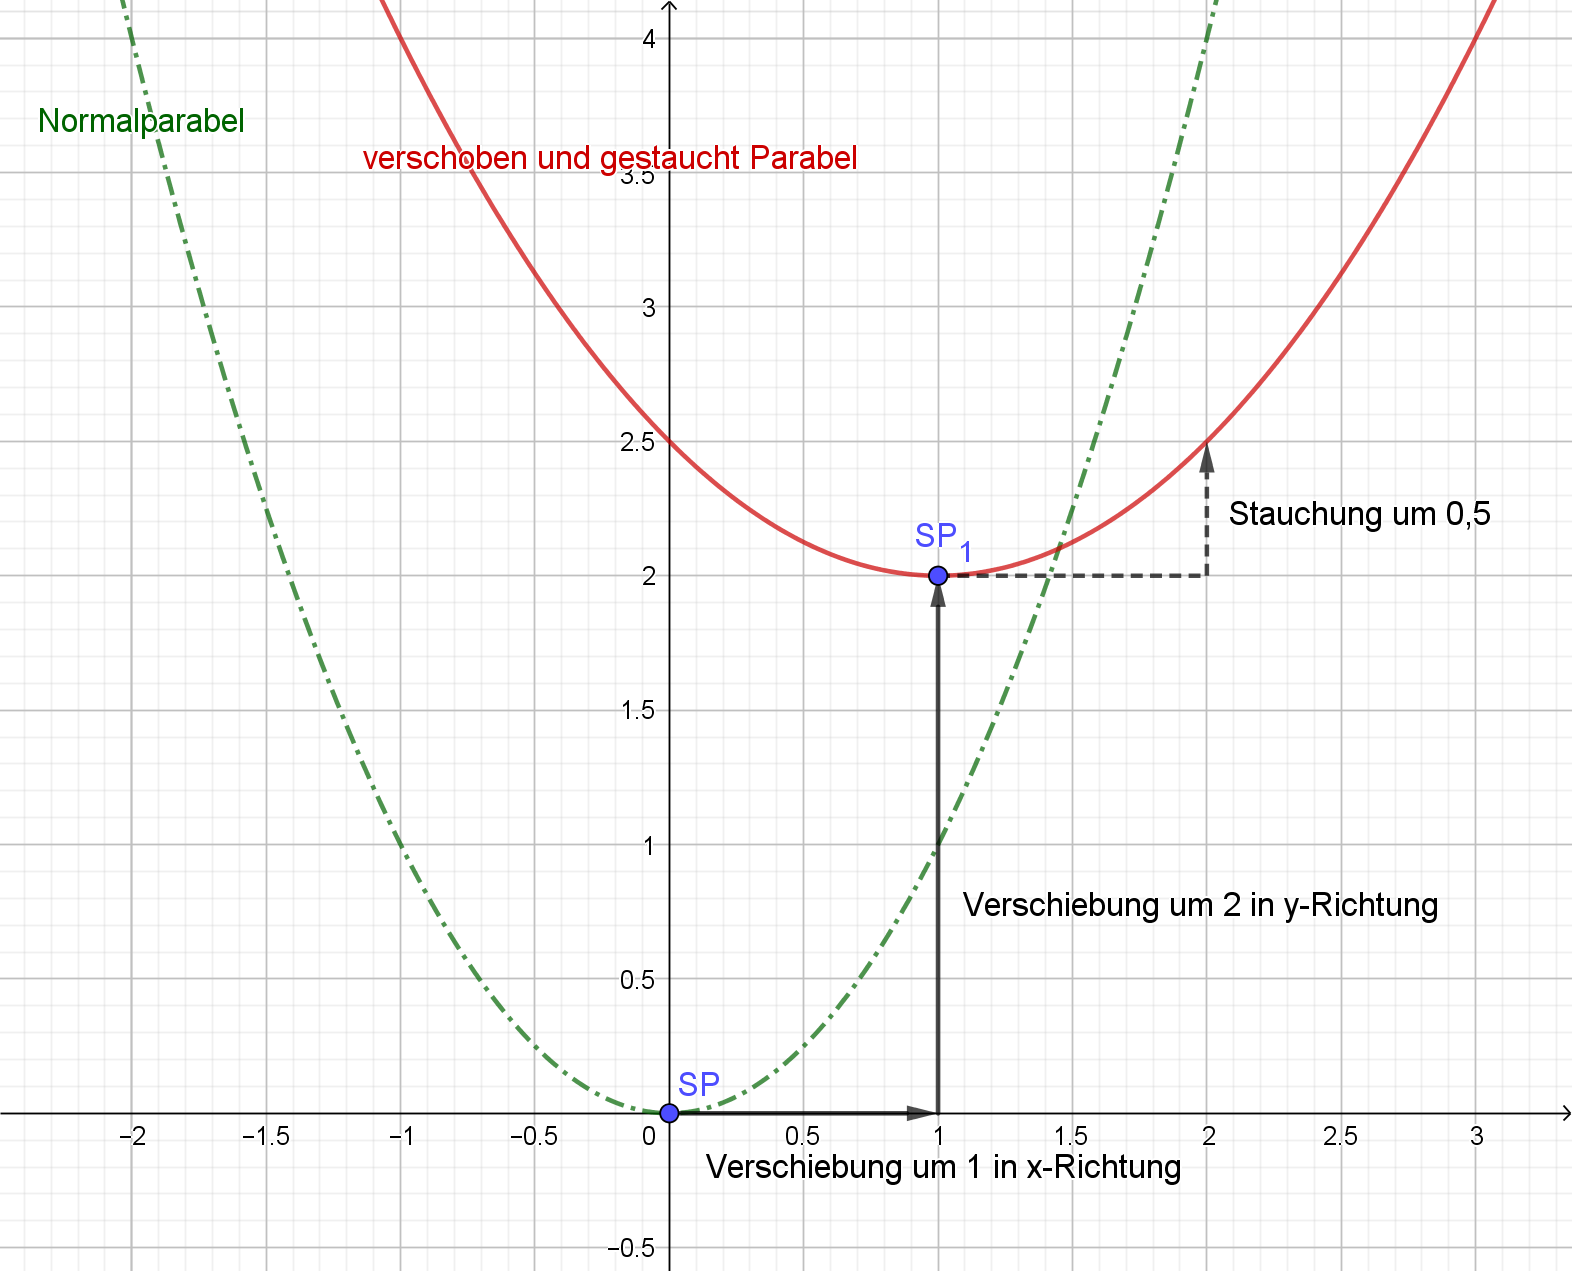
\includegraphics[width=0.48\textwidth]{../99_Bilder/SP_Form.png}\\
		\textbf{Der Streckungsfaktor a}:\\
		(1) Bereits bei der Betrachtung der Scheitelpunktform können wir einiges über den Funktionsgraphen ablesen.\\
		\begin{tabularx}{0.5\textwidth}{XX}
			- Öffnungsrichtung & - Streckung/Stauchung
		\end{tabularx}
		\par\noindent
		\begin{tabularx}{0.5\textwidth}{l|l|l}
			\diagbox{\(|a|\)}{\(a\)} & \(a > 0\) & \( a < 0\)\\
			\hline
			\(|a| < 1\) & nach oben geöffnet & nach unten geöffnet\\
			& gestaucht & gestaucht\\
			\hline
			\(|a|> 1\) & nach oben geöffnet & nach unten geöffnet\\
			& gestreckt & gestreckt
		\end{tabularx}\\
		\par\bigskip\noindent
		\begin{tabularx}{0.5\textwidth}{XX}
			\includegraphics[width=0.22\textwidth, align=t]{../99_Bilder/a_graph.png} & (2) Haben wir hingegen die Parabel gegeben, können wir an dieser auch einiges über unseren Streckungsfaktor \(a\) ablesen.
		\end{tabularx}\\
		\par\noindent
		Daraus ergibt sich: \(a = 0,5\)\\
		\par\bigskip\noindent
		Haben wir lediglich den Scheitelpunkt sowie einen beliebigen weiteren Punkt gegeben, müssen wir den Streckungsfaktor rechnerisch bestimmen.\\
		Wir stellen die Scheitelpunktform auf und setzen den weiteren Punkt in diese ein, lösen anschließend nach dem Parameter \(a\) auf.\\
		\par\bigskip\noindent
		\underline{Beispiel:} \(SP(1|2), A(3|4)\)\\
		So ergibt sich \(f(x) = a\cdot(x-1)^2+2\). In diese setzen wir die Koordinaten des weiteren Punktes:\\
		\begin{tabularx}{0.5\textwidth}{ll}
			\(4 = a\cdot(3-1)^2 +2\)\\
			\(4 = a\cdot(2)^2 + 2\)\\
			\(4 = 4a +2\) & |\(-2\)\\
			\(2 = 4a\) & |\(:4\)\\
			\(0,5 = a\)
		\end{tabularx}
		\subsection*{Die Linearfaktorform (LFF)}
		Der nächste Prototyp einer quadratischen Funktion ist die \textbf{Linearfaktorform}. Für sie gilt: \(f_{LFF}(x) = a\cdot(x-X_1)\cdot(x-x_2)\ \hat{=}\ a\cdot(x-\text{Nullstelle}_1)\cdot(x-\text{Nullstelle}_2)\).\\
		Zu beachten ist: Die Linearfaktorform kann nur angewendet werden, wenn die Parabel bzw. die quadratische Funktion Nullstellen hat.\\
		\par\noindent
		\begin{tabularx}{0.5\textwidth}{XX}
			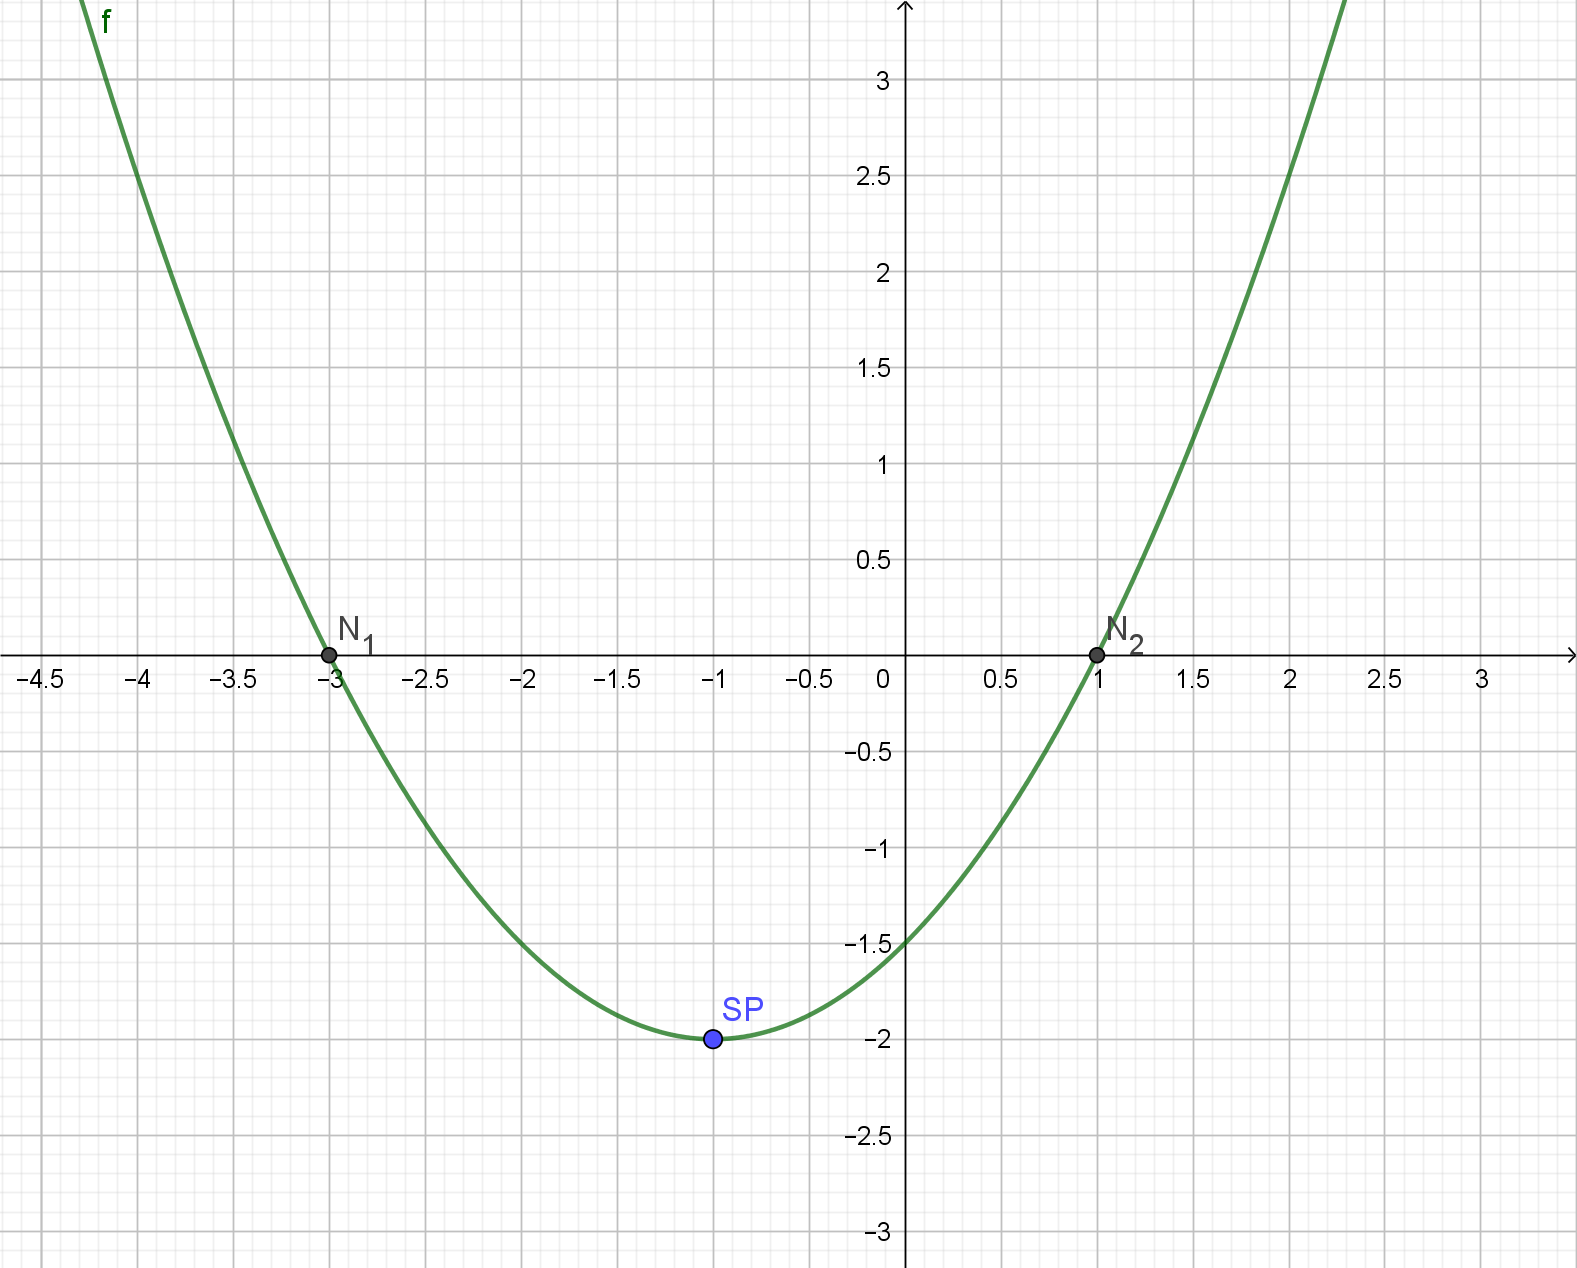
\includegraphics[width=0.23\textwidth,align=t]{../99_Bilder/LFF_Y.png} & \(f(x) = 0,5\cdot(x+1)^2 -2 =\) \(0,5x^2 +x -1,5\ \hat{=}\) \colorbox{green!10}{\(0,5(x+3)(x-1)\)} ist die dazugehörige Linearfaktorform.\\
			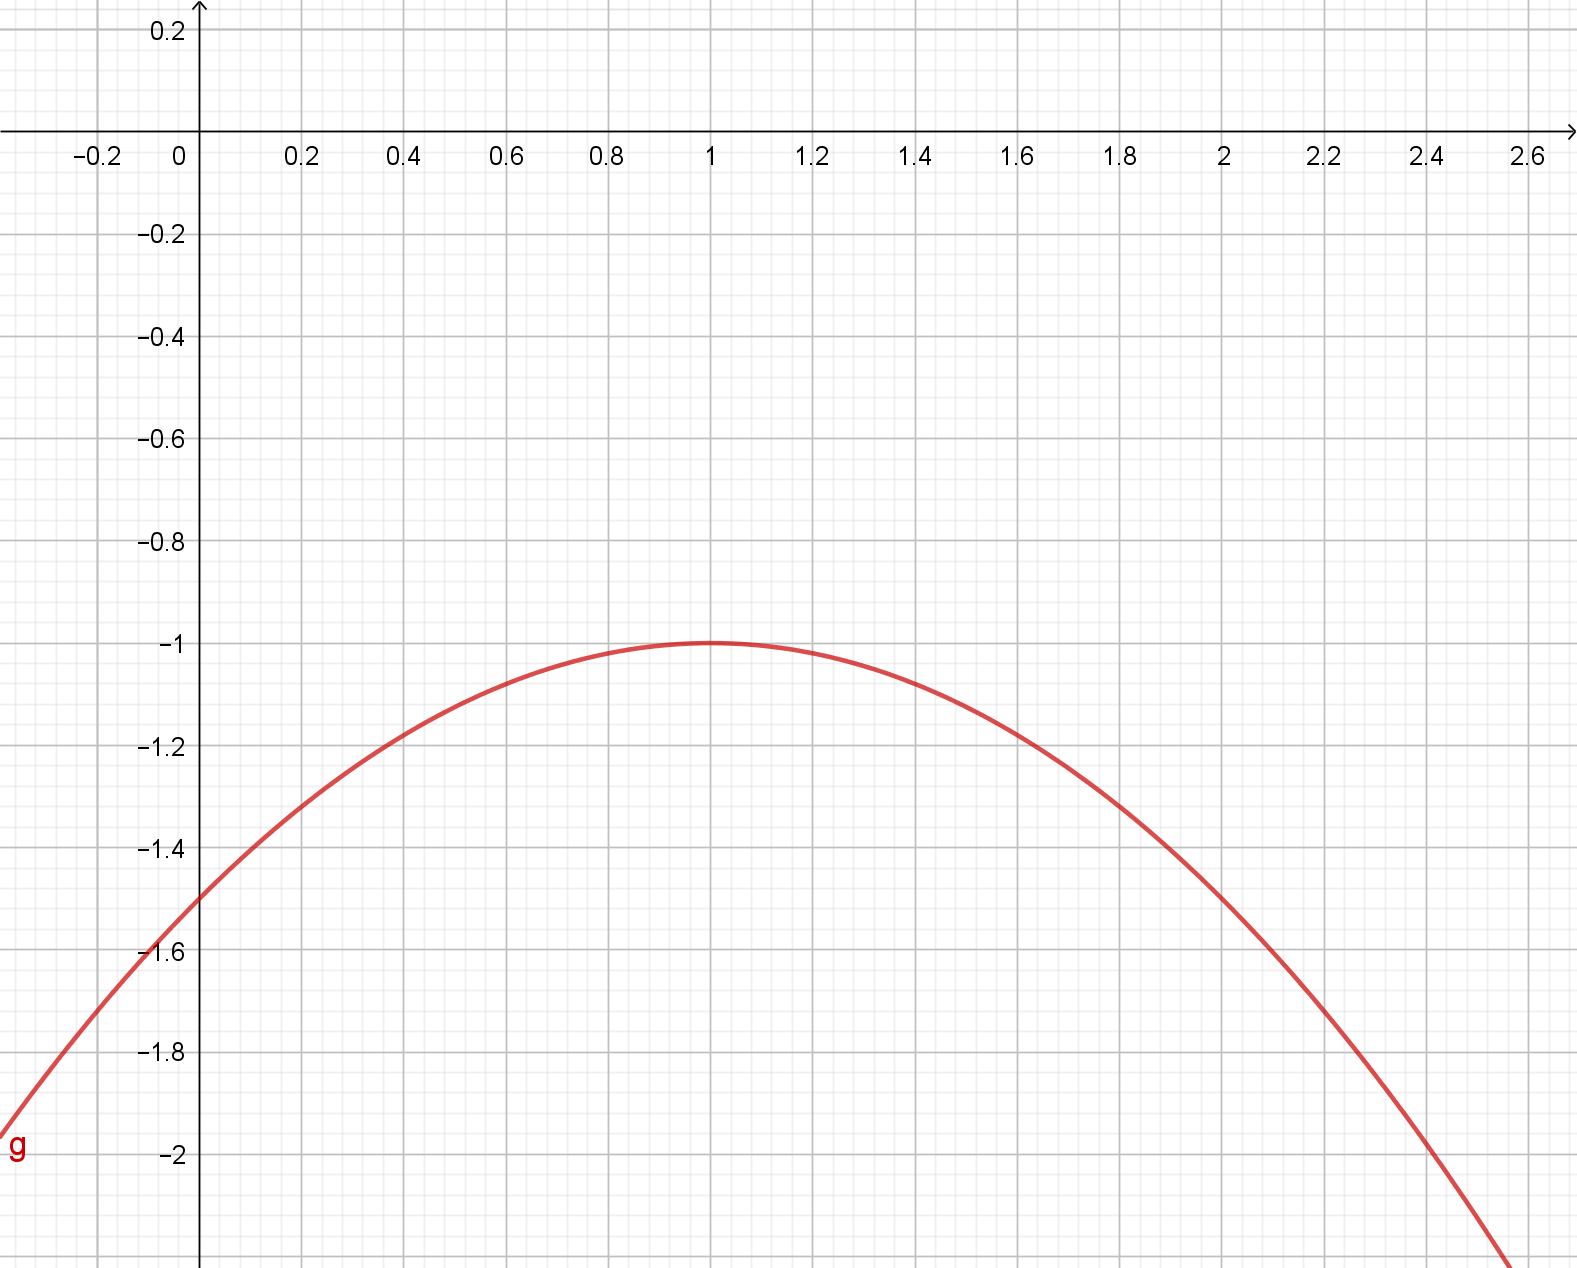
\includegraphics[width=0.23\textwidth,align=t]{../99_Bilder/LFF_N.png} & \(f(x) = -0,5x^2 +x -1,5\) Diese Parabel hat \underline{keine} Linearfaktorform, da sie \underline{keine Nullstellen} besitzt.\\
		\end{tabularx}\\
		\par\noindent
		\textbf{Der Streckungsfaktor a}:\\
		Auch hier gilt: sind die Nullstellen sowie ein weiterer Punkt bekannt, können wir den Streckungsfaktor \(a\) bestimmen.\\
		\par\noindent
		Hierfür stellen wir die Linearfaktorform unter Verwendung der gegebenen Nullstellen auf, setzen die Koordinaten des weiteren Punkts ein und lösen nach dem Parameter a.\\
		\par\noindent
		\underline{Beispiel:} \(N_1(-3|0), N_2(1|0); P(-1|-2)\)\\
		\begin{tabularx}{0.5\textwidth}{ll}
			\(f(x) = a\cdot(x+3)(x-1)\) & P einsetzen\\
			\(-2 = a(-1+3)(-1-1)\)\\
			\(-2 = a\cdot(2)\cdot(-2)\)\\
			\(-2 = -4a\) & |\(:(-4)\)\\
			\(0,5 = a\)
		\end{tabularx}
		\subsubsection*{Die allgemeine Form (AF)}
		Der dritte Prototyp ist die \textbf{allgemeine Form}. Bei ihr gilt: \(f_{AF}(x) = ax^2 +bx+c\).\\
		Diese Form erhält man, wenn man die Scheitelpunkt- oder die Linearfaktorform ausmultipliziert.
		\subsubsection*{Die Normalform (NF)}
		Bei der \textbf{Normalform} handelt es sich um eine spezielle Schreibweise der Allgemeinen Form. Bei dieser wurde der Leitkoeffizient, also der Koeffizient des \(x^2\) ausgeklammert.
		\begin{align*}
			& f_{AF}(x) = ax^2 +bx + c\\
			\Rightarrow & f(x) = a\cdot(x^2 + \underbrace{\frac{b}{a}}_{p}x + \underbrace{\frac{c}{a}}_{q})\\
			\Rightarrow & f_{NF}(x) = a\cdot(x^2 + px + q)
		\end{align*}
		\subsection{Wechsel zwischen den Prototypen}
		Nachfolgend werden wir uns näher damit beschäftigen, wie man zwischen den verschiedenen Darstellungsformen wechselt.\\
		\underline{Beachte:} Der Streckungsfaktor \(a\) kann in allen Prototypen äquivalent verwendet werden.
		\subsubsection*{SPF \(\Rightarrow\) AF / LFF \(\Rightarrow\) AF}
		Gegeben ist eine quadratische Funktion in \textit{Scheitelpunktform}. Um diese in die \textit{allgemeine Form} zu überführen muss lediglich ausmultipliziert und gleiche Terme zusammengefasst werden.\\
		\par\noindent
		\begin{align*}
			& f_{SPF}(x) = a(x-x_s)^2+y_s\\
			\Rightarrow & f(x) = a(x^2-2x_sx +x_s^2) + y_s\\
			\Rightarrow & f(x) = ax^2 \underbrace{-2ax_s}_{b}x + \underbrace{ax_s^2+y_s}_{c}\\
			\Rightarrow & f_{AF}(x) = ax^2+bx+c
		\end{align*}
		Das gleiche Vorgehen wenden wir an, wenn die \textit{Linearfaktorform} gegeben ist und wir diese in die \textit{allgemeine Funktion} überführen wollen.\\
		\par\noindent
		\begin{align*}
			& f_{LFF}(x) = a(x-x_1)(x-x_2)\\
			\Rightarrow & f(x) = a(x^2-x_1x - x_2x +x_1x_2)\\
			\Rightarrow & f(x) = ax^2-ax_1x - ax_2x +ax_1x_2\\
			\Rightarrow & f(x) = ax^2 + \underbrace{(-ax_1-ax_2)}_{b}x \underbrace{+x_1x_2}_{c}\\
			\Rightarrow & f_{AF}(x) = ax^2+bx+c
		\end{align*}
		\subsubsection*{AF \(\Rightarrow\) LFF}
		Haben wir eine quadratische Funktion in \textit{allgemeiner Form}, so können wir diese in \textit{Linearfaktorform} überführen, wenn sie Nullstellen besitzt.\\
		Zunächst bestimmen wir den Streckungsfaktor - der Faktor, der in den vorhandenen Koeffizienten steckt. Nachdem wir diesen \grq{}extrahiert\grq{} haben, wollen wir den übrigen Term faktorisieren. Hierfür haben wir diverse Möglichkeiten. Faktorisieren durch...
		\begin{itemize}
			\item Gruppieren
			\item teilen und schieben
			\item Nullstellenberechnung 
		\end{itemize}
		\tiny{(Als Referenz für die verschiedenen Vorgehensweisen: 02.1\_Faktorisieren)}
		\normalsize
		\subsubsection*{LFF \(\Rightarrow\) SPF}
		Um eine quadratische Funktion aus der \textit{Linearfaktorform} in die \textit{Scheitelpunktform} zu überführen, können wir uns zu nutze machen, dass die x-Stelle des Scheitelpunkts mittig zwischen den beiden Nullstellen liegt. \(\Rightarrow x_s = \frac{x_1+x_2}{2}\).\\
		Um \(y_s\) zu bestimmen, setzen wir die Koordinaten eines Nullpunktes in die Funktion ein und lösen nach \(y_s\).\\
		\par\noindent
		\underline{Beispiel:} \(f_{LFF}(x) = 0,5\cdot(x-1)\cdot(x-5)\)\\
		Wir wissen, dass wir den Streckungsfaktor \(a = 0,5\) beibehalten können.\\
		Wir bestimmen \(x_s = \frac{1+5}{2} = 3\).\\
		\(\Rightarrow f_{SPF}(x) = 0,5\cdot(x-3)^2 + y_s\)\\
		\par\noindent
		Es fehlt uns noch \(y_s\). Wir wählen eine der beiden Nullstellen (\(N_1(1|0)\ N_2(5|0)\) und setzen die Koordinaten des Punktes in die Funktion ein.\\
		\par\noindent
		\begin{tabularx}{0.5\textwidth}{ll}
			\(0 = 0,5\cdot(1-3)^2 + y_s\) & |\(AM\)\\
			\(0 = 0,5\cdot\underbrace{(-2)^2}_{4} + y_s\)\\
			\(0 = 2 +y_s\) & |\(-2\)\\
			\(y_s = -2\)
		\end{tabularx}\\
		\par\noindent
		Daraus ergibt sich die folgende Funktion: \[f_{SPF}(x) = 0,5\cdot(x-3)^2-2\]
		\subsubsection*{AF \(\Rightarrow\) SPF}
		Für die Überführung der \textit{allgemeinen Form} in die \textit{Scheitelpunktform} wenden wir ein Vorgehen an, das man \textbf{Quadratische Ergänzung} nennt. \tiny{(Siehe hierzu 02.2\_Quadratische Ergänzung)}\normalsize\\
		\par\noindent
		\underline{Beispiel:} \(f(x) = 5x^2+30x +10\)
		\begin{align*}
			& f(x) = 5x^2+30x+10\\
			\Leftrightarrow & f(x) = 5\cdot(x^2+6x+2)\\
			\Leftrightarrow & = 5\cdot(x^2+2\cdot{}3x+2)\\
			\Leftrightarrow & = 5\cdot(x^2+2\cdot{}3x \underbrace{+ 3^2 - 3^2}_{\text{Addition von }0} +2)\\
			\Leftrightarrow & = 5\cdot(x^2 +2\cdot{}3x + 3^2\ \ \ \ \underbrace{- 3^2 +2}_{-7})\\
			\Leftrightarrow & = 5\cdot\underbrace{(x^2 + 2\cdot{}3x + 3^2)}_{1. Binomische Formel} +5\cdot(-7)\\
			\Leftrightarrow & = 5\cdot(x+3)^2 -35
		\end{align*}
		Die Scheitelpunktform für \(f(x) = 5x^2+30x+10\) ist also \colorbox{green!10}{\(f(x) = 5(x+3)^2 - 35\)}
	\end{worksheet}
\end{document}